\documentclass[12pt]{article}

% Essential packages
\usepackage[utf8]{inputenc}
\usepackage[T1]{fontenc}
\usepackage{amsmath}
\usepackage{mathtools}
\usepackage{graphicx}
\usepackage[margin=1in]{geometry}
\usepackage{algorithmic}
\usepackage{algorithm}
\usepackage{centering}
\usepackage{svg}
\usepackage{amssymb}

% Document information
\title{Tarea 2 - Análisis de algoritmos}
\author{David Rivera Morales \\ 320176876 \and José Antonio Gallegos Cortes \\ 320316566}
\date{\today}

\begin{document}

% Cover page
\begin{titlepage}
\begin{center}

% UNAM Logo
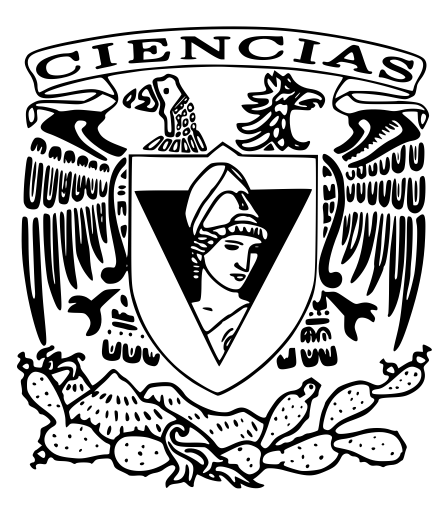
\includegraphics[width=0.3\textwidth]{images/escudo-unam.png}

\vspace{1cm}
{\Large UNIVERSIDAD NACIONAL AUTÓNOMA DE MÉXICO}

\vspace{1.5cm}
{\Large FACULTAD DE CIENCIAS}

\vspace{3cm}
{\Large Tarea 2}\\
\vspace{0.5cm}
{\Large Análisis de algoritmos}

\vspace{2cm}
\vspace{0.5cm}
{\large Rivera Morales David}\\
{\large 320176876}\\
\vspace{0.5cm}
{\large Gallegos Cortes José Antonio}\\
{\large 320316566}

\vfill
{\large \today}
\end{center}
\end{titlepage}

\section*{Solución de los 8 pares de funciones}

% Nota: Recordamos que para el análisis asintótico se considera el comportamiento cuando \( n \to \infty \).

\begin{enumerate}

  \item \textbf{Par 1:} 
  % Definición de las funciones f(n) y g(n).
  \[
    f(n) = \log(n^2), \quad g(n) = \log\bigl(n^2 + 1\bigr).
  \]
  % Explicación paso a paso:
  % 1. Se observa que para n grande, el término 1 en n^2 + 1 es insignificante respecto a n^2.
  % 2. Por ello, se tiene que \( n^2 + 1 \sim n^2 \) cuando \( n \to \infty \).
  % 3. Usando la propiedad de los logaritmos: \(\log(n^2) = 2\log(n)\).
  % 4. Así, ambos términos se comportan como \(2\log(n)\) para n suficientemente grande.
  % 5. Al formar el cociente, se obtiene una constante positiva, lo que implica que f(n) y g(n) tienen el mismo orden de crecimiento.
  \textbf{Análisis:} Para \(n\) grande,
  \[
    n^2 + 1 \sim n^2 \quad \Longrightarrow \quad \log\bigl(n^2 + 1\bigr) \sim \log(n^2) = 2\log(n).
  \]
  Por lo tanto,
  \[
    \frac{\log(n^2)}{\log\bigl(n^2 + 1\bigr)} \; \xrightarrow[n \to \infty]{} \; \text{constante positiva},
  \]
  lo que nos permite concluir que:
  \[
    f(n) \in \Theta\bigl(g(n)\bigr).
  \]

  \item \textbf{Par 2:} 
  % Definición de las funciones.
  \[
    f(n) = \log(n), \quad g(n) = \log(n^2).
  \]
  % Explicación:
  % 1. Aplicamos la propiedad logarítmica: \(\log(n^2)= 2\log(n)\).
  % 2. Así, g(n) es simplemente 2 veces f(n), es decir, un múltiplo constante de f(n).
  % 3. Al calcular el cociente, se obtiene \(\frac{1}{2}\), lo que es una constante positiva.
  \textbf{Análisis:}
  \[
    \log(n^2)= 2\log(n) \quad \Longrightarrow \quad \frac{f(n)}{g(n)} = \frac{\log(n)}{2\log(n)} = \frac{1}{2}.
  \]
  Por ello,
  \[
    f(n) \in \Theta\bigl(g(n)\bigr).
  \]

  \item \textbf{Par 3:} 
  % Definición de las funciones.
  \[
    f(n) = (n^3)^2 = n^6, \quad g(n) = n^3.
  \]
  % Explicación:
  % 1. Se observa que \(n^6\) es \(n^3\) elevado al cuadrado, por lo que crece mucho más rápido que \(n^3\).
  % 2. Al formar el cociente se tiene:
  \[
    \frac{f(n)}{g(n)} = \frac{n^6}{n^3} = n^3.
  \]
  % 3. Como \(n^3 \to \infty\) cuando \(n \to \infty\), se concluye que f(n) crece asintóticamente mucho más rápido que g(n).
  \textbf{Análisis:}
  \[
    \frac{n^6}{n^3} = n^3 \xrightarrow[n \to \infty]{} \infty.
  \]
  Por lo tanto,
  \[
    f(n) \in \omega\bigl(g(n)\bigr).
  \]

  \item \textbf{Par 4:} 
  % Definición de las funciones.
  \[
    f(n) = n \,\log(n^2), \quad g(n) = n \,\log(n).
  \]
  % Explicación:
  % 1. Se aplica la propiedad logarítmica: \(\log(n^2)= 2\log(n)\), obteniéndose:
  \[
    f(n) = n \cdot 2\log(n)= 2n\log(n).
  \]
  % 2. Como g(n) = n log(n), el cociente es:
  \[
    \frac{f(n)}{g(n)} = \frac{2n\log(n)}{n\log(n)} = 2.
  \]
  % 3. El cociente constante implica que ambas funciones tienen el mismo orden de crecimiento.
  \textbf{Análisis:}
  \[
    f(n) \in \Theta\bigl(g(n)\bigr).
  \]

  \item \textbf{Par 5:}
  % Definición de las funciones.
  \[
    f(n) = \log\bigl(\log(n)\bigr), \quad g(n) = \sqrt{\log(n)}.
  \]
  % Explicación:
  % 1. La función \(\log(n)\) tiende a infinito al crecer \(n\), pero de manera lenta.
  % 2. La función \(f(n)\) toma el logaritmo de \(\log(n)\), lo que ralentiza aún más su crecimiento.
  % 3. En cambio, \(g(n)=\sqrt{\log(n)}\) equivale a \((\log(n))^{1/2}\), que crece más rápido que \(\log(\log(n))\).
  % 4. Para ver esto, se forma el cociente:
  \[
    \frac{f(n)}{g(n)} = \frac{\log(\log(n))}{(\log(n))^{1/2}}.
  \]
  % 5. Al tomar el límite cuando \(n \to \infty\), el denominador domina al numerador, y el límite es 0.
  \textbf{Análisis:}
  \[
    \lim_{n \to \infty} \frac{\log(\log(n))}{(\log(n))^{1/2}} = 0.
  \]
  % Concluimos que f(n) crece mucho más despacio que g(n).
  \[
    f(n) \in o\bigl(g(n)\bigr).
  \]

  \item \textbf{Par 6:}
  % Definición de las funciones.
  \[
    f(n) = n^{\log(n)}, \quad g(n) = n \,\log(n) - n.
  \]
  % Explicación:
  % 1. Se simplifica g(n) factorizando n: 
  \[
    g(n) = n\bigl(\log(n)-1\bigr).
  \]
  % 2. Para n grande, \(\log(n)-1\) es positivo, por lo que g(n) se comporta como \(n\log(n)\).
  % 3. Para f(n), se utiliza la transformación exponencial:
  \[
    n^{\log(n)} = \exp\bigl(\log(n)\cdot\log(n)\bigr)= \exp\bigl((\log(n))^2\bigr).
  \]
  % 4. Se compara el crecimiento de \(\exp\bigl((\log(n))^2\bigr)\) con \(n\log(n)\) formando el cociente:
  \[
    \frac{f(n)}{g(n)} \approx \frac{\exp\bigl((\log(n))^2\bigr)}{n\,\log(n)}.
  \]
  % 5. Tomando logaritmos del cociente para simplificar la comparación:
  \[
    \log\!\Bigl(\frac{f(n)}{g(n)}\Bigr) \approx (\log(n))^2 - \log\bigl(n\,\log(n)\bigr).
  \]
  % 6. Se nota que \((\log(n))^2\) domina a \(\log(n) + \log(\log(n))\) (recordando que \(\log\bigl(n\,\log(n)\bigr) = \log(n) + \log(\log(n))\)).
  % 7. Esto implica que el cociente tiende a infinito, demostrando que f(n) crece mucho más rápido que g(n).
  \textbf{Análisis:}
  \[
    \lim_{n\to\infty} \frac{f(n)}{g(n)} = \infty.
  \]
  Por lo tanto,
  \[
    f(n) \in \omega\bigl(g(n)\bigr).
  \]

  \item \textbf{Par 7:}
  % Definición de las funciones.
  \[
    f(n) = \log\bigl(n^{\,n \log n}\bigr), \quad g(n) = \sqrt{n \,\log(n)}.
  \]
  % Explicación:
  % 1. Aplicamos la propiedad logarítmica para f(n): 
  \[
    \log\bigl(n^{\,n \log n}\bigr) = n \log n \cdot \log n = n\,(\log n)^2.
  \]
  % 2. Se reescribe g(n) en forma de potencias:
  \[
    g(n) = \sqrt{n\,\log(n)} = (n\,\log(n))^{1/2} = n^{1/2}\,(\log(n))^{1/2}.
  \]
  % 3. Se forma el cociente:
  \[
    \frac{f(n)}{g(n)} = \frac{n\,(\log(n))^2}{n^{1/2}\,(\log(n))^{1/2}} = n^{1/2}\,(\log(n))^{3/2}.
  \]
  % 4. Dado que tanto \(n^{1/2}\) como \((\log(n))^{3/2}\) tienden a infinito al crecer n, su producto también lo hace.
  \textbf{Análisis:}
  \[
    \lim_{n \to \infty} n^{1/2}\,(\log(n))^{3/2} = \infty.
  \]
  Así,
  \[
    f(n) \in \omega\bigl(g(n)\bigr).
  \]

  \item \textbf{Par 8:}
  % Definición de las funciones.
  \[
    f(n) = 2^{\,n^2 + 1}, \quad g(n) = 4^n.
  \]
  % Explicación:
  % 1. Se reescribe \(g(n)\) en base 2 utilizando que \(4 = 2^2\):
  \[
    4^n = (2^2)^n = 2^{2n}.
  \]
  % 2. Así, f(n) se expresa como \(2^{\,n^2+1}\) y g(n) como \(2^{2n}\).
  % 3. Se comparan los exponentes: \(n^2 + 1\) crece mucho más rápido que \(2n\) para n grande.
  % 4. Al formar el cociente:
  \[
    \frac{f(n)}{g(n)} = \frac{2^{n^2+1}}{2^{2n}} = 2^{\,n^2 + 1 - 2n}.
  \]
  % 5. Se simplifica el exponente:
  \[
    n^2 + 1 - 2n = n^2 - 2n + 1 = (n-1)^2.
  \]
  % 6. Como \((n-1)^2\) tiende a infinito, \(2^{(n-1)^2}\) también lo hace, lo que implica que f(n) crece asintóticamente más rápido.
  \textbf{Análisis:}
  \[
    f(n) \in \omega\bigl(g(n)\bigr).
  \]

\end{enumerate}

\end{document}
